\documentclass[a4paper,11pt]{scrartcl}

\usepackage[ngerman]{babel}
\usepackage[T1]{fontenc}
\usepackage[utf8]{inputenc}
\usepackage{ebgaramond}
\usepackage{helvet}
\usepackage{graphicx}
\usepackage{apacite}
\usepackage[hyphens]{url}

\begin{document}

\title{DRM}
\subtitle{Encrypted Media Extensions}
\author{Patrick Bucher}
\maketitle

\tableofcontents

\section{DRM}

Digitel Rights Management, Digital Restriction Management...

\section{Encrypted Media Extensions}

\subsection{Motivation}

Mit HTML5 ist es möglich, Video- und Audiodateien ohne Plugins wie Adobe Flash und Microsoft Silverlight direkt im Browser abzuspielen. Das funktioniert für kostenlose Inhalte mittlerweile hervorragend. Das Problem ist aber, dass kostenpflichtige Angebote wie Netflix und Zattoo ihre Videos nur denen zeigen wollen, die vorher bezahlt haben. Das funktioniert mit HTML5-Video-Tags leider nicht. Darum setzen diese komerziellen Angebote weiterhin auf Microsoft Silverlight und Adobe Flash.

Darum haben sich die Leute im W3C gedacht, dass DRM auch Einzug in HTML5 halten soll, um Adobe Flash und Microsoft Silverlight endgültig den Garaus zu machen.

\subsection{Funktionsweise}

Auf der Webseite \cite{w3c} steht alles beschrieben.

\begin{figure}
    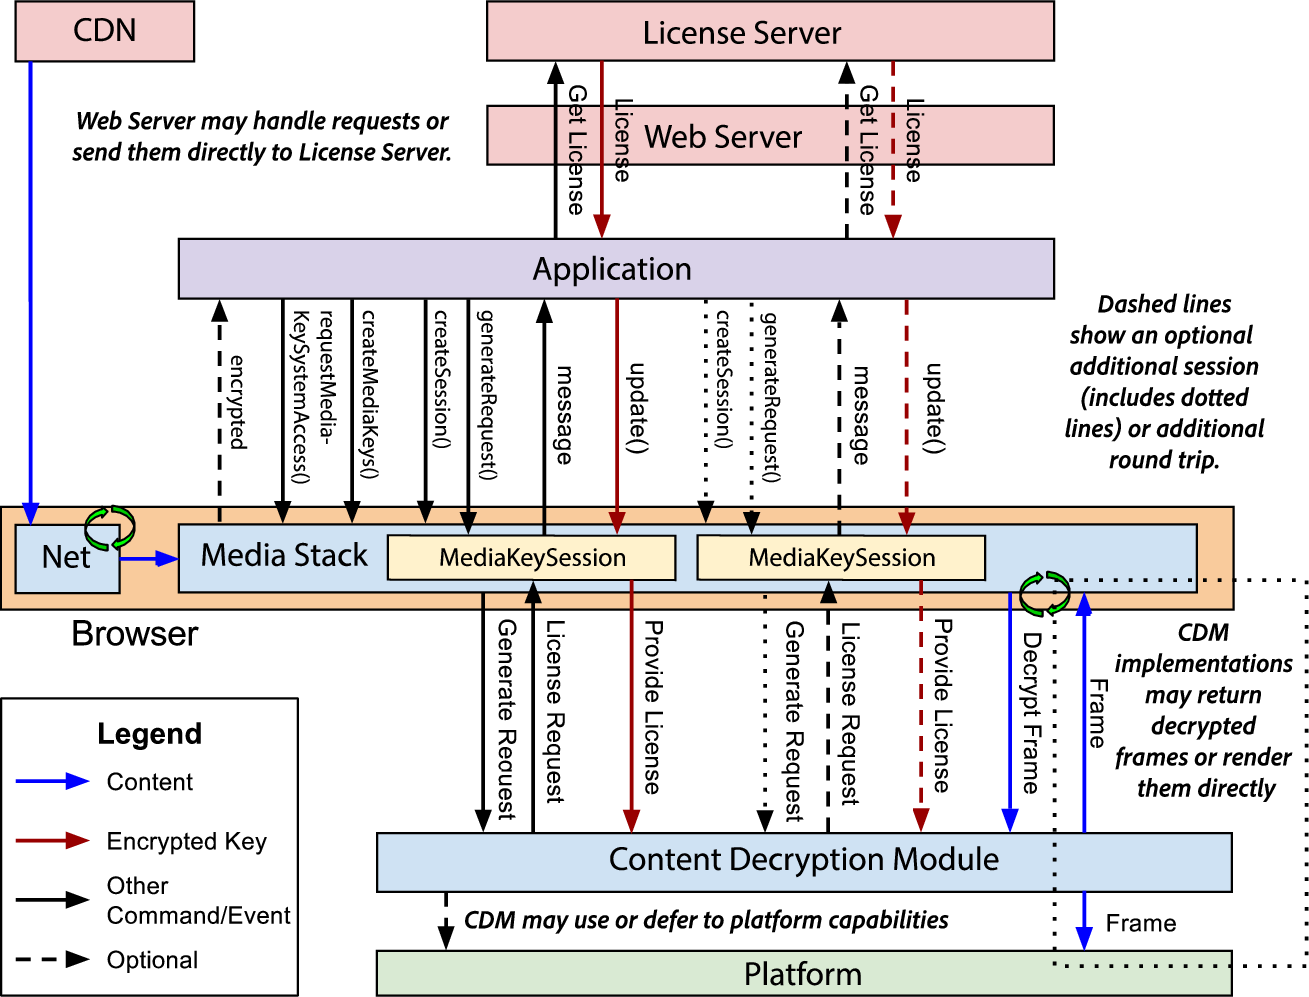
\includegraphics[width=1.0\textwidth]{eme-overview.png}
    \caption{Der EME-Stack\protect\footnotemark}
    \label{fig:EME}
\end{figure}
\footnotetext{Quelle: \url{https://www.w3.org/TR/encrypted-media/stack-overview.svg}}

\subsection{Kontroverse}

Das Problem ist, dass Open-Source-Software keinen proprietären Code enthalten sollte, durch die EME das aber nötig wird.

\section{Fazit}


\bibliography{drm-eme.bib}
\bibliographystyle{apacite}

\end{document}
